The structural-mechanics benchmark put the neural mean and the kernel in the
balanced regime. To see the other regime we apply the same components to the
radiative-transfer emulation problem of \citet{susiluoto2025radiative}: per
spectral band of the OCO-2 instrument, learn the map from a reduced
atmospheric state ($20$--$24$ dimensions after the dimension reduction of
that paper) to the reduced radiance ($40$ PCA coefficients of the
monochromatic spectrum). The OSF project (\texttt{u2t8a}) publishes a training
pool of $20000$ pairs and, separately, $2000$ test states together with the
kernel-flow emulator's own predictions on them; the released overlap check
reports that the two sets share no point. The recorded runs split the pool
$18000/2000$ into training and validation. Within each run, the validation
split selects network checkpoints, kernel length scales and nuggets, and
the coordinate winners below. The public test states are used for reported
evaluation and subsequent diagnostics. Because this study was developed
through repeated analyses of a public benchmark, its comparisons are
retrospective, not a preregistered confirmatory test. The historical comparison
retains those runs; Section~\ref{sec:oco-grid-sensitivity} reports a separate
matched sensitivity campaign.
The carve is taken from the source study's Sobol training design while the
public test states are a separate draw, and the two differ: the flat
network's mean relative error is $6.7\%$ on the carve against $4.4\%$ on the
test block on O2, so every selection made on the carve is a selection under
a shift between the two, not a same-distribution choice.
The comparison is therefore computed on identical test points against the
published emulator itself rather than against our reimplementation of it.

The two error criteria are defined here on the released reduced
representation. Neither is the source study's instrument-noise or retrieval
acceptance test. Let $z\in\mathbb R^{40}$ contain the standardized
coefficients, let $U$ have the retained orthonormal PCA columns, and put
$D_z=\operatorname{diag}(s_z)$. The stored means and scales reconstruct
\begin{equation}
 R(z)=\mu_y+U(\mu_z+D_z z),\qquad U^\top U=I.
 \label{eq:oco-reconstruction}
\end{equation}
The two reported mean relative errors are
\begin{align}
 E_{\rm red}&=\frac1N\sum_{i=1}^N
       \frac{\|\hat z_i-z_i\|_2}{\|z_i\|_2},
       \label{eq:oco-reduced}\\
 E_{\rm rad}&=\frac1N\sum_{i=1}^N
       \frac{\|D_z(\hat z_i-z_i)\|_2}{\|R(z_i)\|_2}.
       \label{eq:oco-radiance}
\end{align}
Orthogonality gives $\|R(\hat z)-R(z)\|_2
=\|D_z(\hat z-z)\|_2$; the reconstruction offsets cancel in the
numerator but remain in the denominator. The radiance criterion compares
two forty-component reconstructions, so it excludes PCA truncation error,
the instrument line shape, and the measurement-noise model. Its numerator
weights concentrate on the leading coefficients.

For fixed nonnegative weights $\omega_i,a_j$, the squared objective
$N^{-1}\sum_{i,j}\omega_i a_j(\hat z_{ij}-z_{ij})^2$ separates by
coordinate. Ordinary coordinatewise RMSE selection minimizes this
objective with $\omega_i=a_j=1$. Squared relative coefficient error instead
uses $\omega_i=\|z_i\|_2^{-2}$; squared relative radiance error uses
$\omega_i=\|R(z_i)\|_2^{-2}$ and $a_j=s_{z,j}^2$. Fixed per-sample
denominators therefore preserve separability for the squared objectives,
although they can change the winning member. The square root in each
summand of \eqref{eq:oco-reduced}--\eqref{eq:oco-radiance} couples
coordinates, so coordinatewise selection need not minimize either reported
mean norm, or both simultaneously.

\begin{table}[t]
\centering
\caption{OCO-2 O2 band, scored on the $2000$ public test states, which are
disjoint from the training pool; within-run selection used a validation
split of the pool. Every fitted row is mean $\pm$ standard deviation over ten
seeds; neural networks use a matched $250$-epoch budget. The
kernel-flow row is the emulator of \citet{susiluoto2025radiative}, scored
from its own stored predictions on fixed test points, and is identical at
every seed. ``Features'' means the penultimate
activations of the trained network; the kernel head is the same exact
Mat\'ern solve as everywhere else in this paper, and the two raw-input rows
are fit by that same kernel-tuning routine and budget as the feature heads:
the same scale grid $\{0.5,1,2,4\}$ times the median distance, the same
nugget grid $\{10^{-8},10^{-6},10^{-4}\}$, the same $6000$-sample tuning
subsample, and the winner refit on all $18000$ training points. This matches
the kernel stage, not total computation: feature heads additionally require
neural-network training. The
raw-input rows' selected settings vary from seed to seed; every feature head,
by contrast, selected the largest multiplier ($4$) and the smallest nugget
($10^{-8}$) of that grid at all thirty band-seeds, so the feature-head
numbers describe this finite search grid and do not establish an optimum
over wider grids. The ARD radiance summary includes a bimodal selection
outcome: configurations selected on reduced validation error give
$0.150\%$ radiance error at seven seeds and $0.329\%$ at three.
Entries are aggregated from the original campaign records; the ARD
radiance mean and standard deviation are included here explicitly.}
\label{tab:oco2}
\begin{adjustbox}{max width=\linewidth}
\begin{tabular}{lcc}
\toprule
model & reduced & radiance \\
\midrule
Mat\'ern kernel, raw input, one length scale & $40.57\pm0.10$\% & $0.233\pm0.003$\% \\
Mat\'ern kernel, raw input, sensitivity-scaled (ARD) & $29.98\pm0.15$\% & $0.204\pm0.087$\% \\
kernel-flow emulator \citep{susiluoto2025radiative} & 16.89\% & 0.0448\% \\
residual MLP, flat metric & $4.43\pm0.05$\% & $0.195\pm0.014$\% \\
residual MLP, weighted-coefficient loss & $49.32\pm0.40$\% & $0.0442\pm0.0044$\% \\
residual MLP, exact radiance loss & $59.02\pm0.76$\% & $0.0571\pm0.0057$\% \\
Mat\'ern head on the flat network's features & $4.11\pm0.05$\% & $0.0793\pm0.0072$\% \\
Mat\'ern head on the weighted network's features & $21.70\pm0.52$\% & $0.0319\pm0.0020$\% \\
Mat\'ern head on the radiance network's features & $20.48\pm0.61$\% & $0.0379\pm0.0037$\% \\
per-coordinate combination & $\mathbf{4.12\pm0.05}$\% & $\mathbf{0.0294\pm0.0020}$\% \\
\bottomrule
\end{tabular}
\end{adjustbox}
\end{table}

\begin{table}[t]
\centering
\caption{Readout control for the kernel heads, ten seeds per band, mean
$\pm$ standard deviation over seeds. For the flat and weighted-coefficient
networks the same
frozen last-layer features are read out three ways: by the network's own
trained output layer, by a ridge regression refit on those features with
the penalty chosen on validation, and by the exact Mat\'ern head. The rows
come from the recorded follow-up run of the campaign script with the ridge rows added
(\texttt{campaign/jpl\_seeded.py}; body generated by
\texttt{campaign/gen\_oco\_ridge\_table.py}); the rerun's network and head
rows reproduce Table~\ref{tab:oco2} within the seed spread.}
\label{tab:oco2ridge}
\begin{adjustbox}{max width=\linewidth}
\begin{tabular}{lcc}
\toprule
model & reduced & radiance \\
\midrule
\multicolumn{3}{l}{\emph{O2 band} (10 seeds)} \\
network, flat loss & $4.43\pm0.05$\% & $0.195\pm0.014$\% \\
\quad ridge readout on its frozen features & $4.71\pm0.07$\% & $0.228\pm0.014$\% \\
\quad Mat\'ern head on its frozen features & $4.11\pm0.05$\% & $0.0793\pm0.0072$\% \\
network, weighted-coefficient loss & $49.33\pm0.40$\% & $0.0439\pm0.0031$\% \\
\quad ridge readout on its frozen features & $45.71\pm0.61$\% & $0.0521\pm0.0043$\% \\
\quad Mat\'ern head on its frozen features & $21.72\pm0.52$\% & $0.0316\pm0.0019$\% \\
\multicolumn{3}{l}{\emph{WCO2 band} (10 seeds)} \\
network, flat loss & $16.44\pm0.06$\% & $0.226\pm0.012$\% \\
\quad ridge readout on its frozen features & $16.51\pm0.06$\% & $0.252\pm0.017$\% \\
\quad Mat\'ern head on its frozen features & $16.28\pm0.06$\% & $0.116\pm0.007$\% \\
network, weighted-coefficient loss & $62.57\pm0.56$\% & $0.0738\pm0.0057$\% \\
\quad ridge readout on its frozen features & $61.32\pm0.43$\% & $0.0842\pm0.0067$\% \\
\quad Mat\'ern head on its frozen features & $48.67\pm0.45$\% & $0.0533\pm0.0054$\% \\
\multicolumn{3}{l}{\emph{SCO2 band} (10 seeds)} \\
network, flat loss & $8.23\pm0.02$\% & $0.199\pm0.015$\% \\
\quad ridge readout on its frozen features & $8.33\pm0.03$\% & $0.236\pm0.032$\% \\
\quad Mat\'ern head on its frozen features & $8.08\pm0.01$\% & $0.109\pm0.007$\% \\
network, weighted-coefficient loss & $36.46\pm0.65$\% & $0.0751\pm0.0025$\% \\
\quad ridge readout on its frozen features & $40.10\pm0.91$\% & $0.0866\pm0.0039$\% \\
\quad Mat\'ern head on its frozen features & $15.47\pm0.47$\% & $0.0631\pm0.0037$\% \\
\bottomrule
\end{tabular}
\end{adjustbox}

\end{table}

\begin{figure}[t]
\centering
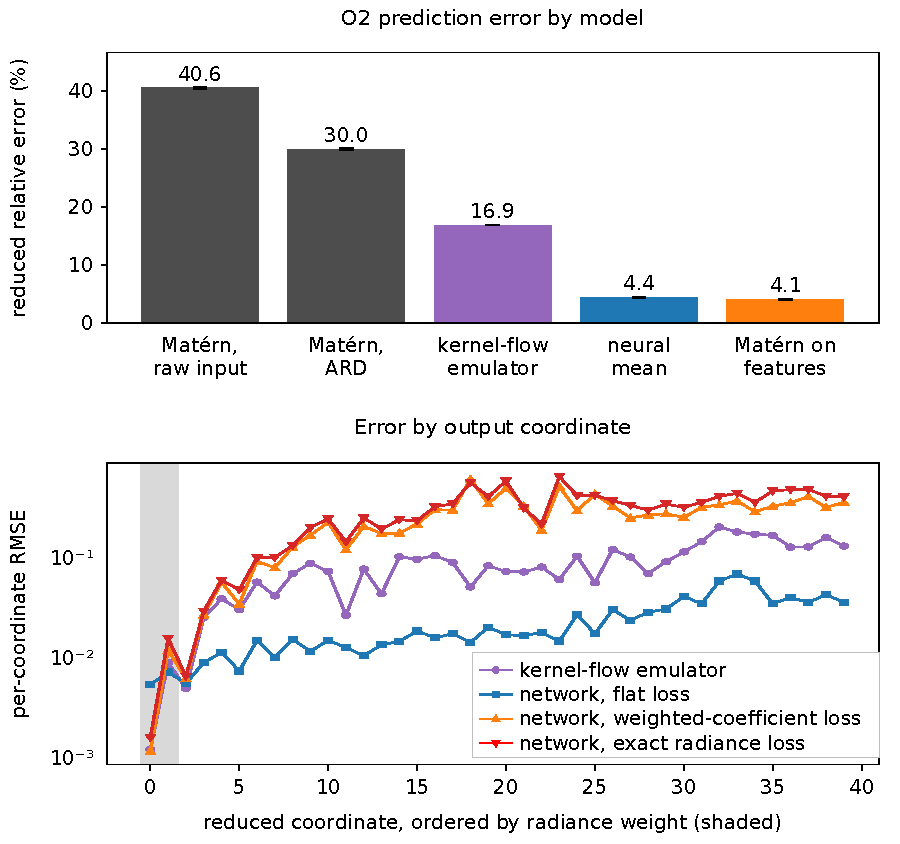
\includegraphics[width=\linewidth]{figs/oco2_seeded.pdf}
\caption{Both panels are drawn from the ten-seed campaign by
\texttt{campaign/make\_oco2\_fig.py}: bars and error bars in the left panel
are the mean and standard deviation over the ten seeds, curves in the right
panel are per-coordinate test RMSE averaged over the same ten. Left: the
representation ladder on the O2 band. The same exact
Mat\'ern machinery moves from $40\%$ on the raw input to $4.1\%$ on the
trained network's features; the kernel-flow emulator and the network sit in
between. Right: per-coordinate test RMSE with the reduced coordinates ordered
by their radiance weight (shaded). Networks are named by the loss they were
trained on. The per-output-tuned kernel-flow
emulator is most accurate exactly on the heavily weighted leading
coefficient ($0.0012$ against the flat network's $0.0054$), while the flat
network is nearly four times more accurate across the trailing thirty
coordinates that the radiance barely sees ($0.0276$ against $0.1037$). Both
weighted losses buy the leading coefficient at the price of the tail, and by
almost the same amount ($0.0012$ and $0.0016$), which is the measurement
behind the reading below; the per-coordinate combination takes
each coordinate from whichever model wins it.}
\label{fig:oco2}
\end{figure}

Table~\ref{tab:oco2} and Figure~\ref{fig:oco2} show the principal comparisons.
The tested kernel routine scores $40\%$ on raw input, $30\%$ after rescaling
each input coordinate by its estimated sensitivity, and $4.1\%$ on the
trained network's features. Under this routine, learned features are more
useful than the raw coordinates or the tested input rescaling. The deep
kernel head is the strongest single model tested on the O2 reduced metric.
Its margin over the network it reads out is $4.11\pm0.05\%$ against
$4.43\pm0.05\%$, and the head has lower error at all ten recorded seeds
on each band.

A linear ridge regression refitted on the same frozen features
(Table~\ref{tab:oco2ridge}) is worse than the network's trained output layer
on the flat-loss network at every band-seed. The Mat\'ern head is better
than both at every band-seed, with a margin over ridge of
$0.60\pm0.07$ percentage points on O2 and about a quarter of a point on
the other bands. Thus this tested linear-refit control does not reproduce
the Mat\'ern improvement; it does not rule out other readout objectives or
optimization procedures. Adding the ridge readouts to coordinate selection
changes the combination by at most $0.002$ percentage points on any band.

Three statements of scope belong next to these numbers. The combination
row is produced by the unweighted selector over the three networks and
their three feature-kernel heads. It takes each reduced
coordinate from the model with the smallest validation root-mean-square
error on that coordinate; the campaign script also runs a selector
weighted by the inverse squared norm of each validation state, the exact
optimizer over the coordinatewise candidate choices of the empirical
squared relative error described by Corollary~\ref{cor:percoordw}, and
it chooses different winners at three seeds on O2 and four on WCO2 yet
changes each band's mean reduced error by less than $0.001$ percentage
points, with unchanged radiance means at the reported precision (both
records are in the release). On O2 the unweighted combination has mean
reduced error $4.11510\%$, slightly above the flat-feature head's
$4.11080\%$, while improving radiance error from $0.07927\%$ to
$0.02940\%$. It therefore does not dominate every individual model on both
criteria. The uncertainty of the
comparison against the emulator is paired: on the same $2000$ test states,
a case-resampling bootstrap of the difference between the combination and
the emulator excludes zero at ten of ten seeds on both metrics on O2 and
SCO2, and at ten of ten on WCO2's reduced metric and nine of ten on its
radiance metric, the exception being the seed that loses by $0.0015$ points;
the seed standard deviations in Table~\ref{tab:oco2} describe retraining
variability, not that comparison. These are descriptive case-resampling
intervals for the recorded predictors, with no adjustment for repeated
benchmark analyses. The claim is confined to what is
rescored: two criteria defined here on the released reduced representation
(the coefficients, and the radiance reconstructed from the retained forty
components), not the full-spectrum acceptance test of
\citet{susiluoto2025radiative}, at a
$250$-epoch budget the networks have not converged at, with the emulator
fitted on $20000$ states against our $18000$ plus a $2000$-state validation
carve. Instrument response, Jacobians and the retrieval itself are not
evaluated, so nothing here says the pipeline is a better OCO-2 emulator
end to end. Learning the metric rather than
setting it by hand does not change this reading. A per-dimension metric fit by
the kernel-flows cross-validation loss of \citet{owhadi2019kernel} reaches the
same $30\%$ on the raw state, and a low-rank Mahalanobis metric with a thousand
more parameters does not improve on it; on the features, where the network has
already conditioned the representation, a learned metric gives no gain over the
isotropic kernel. These observations concern the tested metrics, feature
maps, and tuning budgets; they do not exclude stronger raw-input kernels.

\subsection{What the metric buys, measured}
\label{sec:aniso-measured}
The recorded sweep refits both raw-input kernel rows at five nested
training sizes, ten seeds per band, estimating the sensitivity map from
the available training rows at each size. At $n=18000$ the isotropic-to-adapted
error ratios range from $1.1$ to $1.5$. The fitted log--log slopes differ
little on O2 and more on strong CO$_2$; the numerical results are in
Section~S7. These slopes summarize a finite range of training sizes and
are not asymptotic rates. Proposition~\ref{prop:aniso} instead gives a
conditional finite-design bound for rank truncation; this sweep does not
verify its Lipschitz or native-space assumptions.
\subsection{Retrospective transfer of the two-member rule}
\label{sec:secmom-margin}
Part~(i) of Proposition~\ref{prop:secmom} says that a weaker member helps
the optimal two-member squared-relative-error mixture exactly when
$\varrho<e_1/e_2$. We examine this criterion retrospectively using stored
validation and test predictions for eight models: the two raw-input
kernels, three networks, and three feature-kernel heads. There are
$\binom{8}{2}=28$ pairs at each of thirty band-seeds, $840$ in all.
This diagnostic is not a preregistered member-admission experiment.

Evaluating both sides on the same block, the criterion agrees with whether
the optimal convex mix beats the better member on all $840$ pairs. This
checks an algebraic identity against stored predictions; it is not
independent statistical evidence for the proposition.

The separate transfer question uses $\varrho$ and $e_1/e_2$ estimated
on validation, then compares that verdict with the test-block result.
The test-side outcome is
whether the optimal convex two-member mix beats the better of the two members
\emph{on test}, whichever that is (the order of a pair flips between the
splits in $40$ of the $840$). The rule is correct on $62.4\%$ of the $840$
pairs. Stratified by the observed margin
$|\varrho-e_1/e_2|$ that the rule must resolve, the outcome is
$101$ of $257$ below $0.02$, $95$ of $215$ from $0.02$ to $0.05$, $81$ of
$88$ from $0.05$ to $0.10$, $215$ of $248$ from $0.10$ to $0.25$, and $32$
of $32$ above $0.25$ --- that is $39\%$, $44\%$, $92\%$, $87\%$ and
$100\%$. That scores the existence of a helpful mix. Scoring what the rule
would ship --- the mix at the weight fitted on validation, against the better
test member --- the counts are $142$ of $257$, $107$ of $215$, $76$ of $88$,
$125$ of $248$ and $31$ of $32$ ($57.3\%$ overall). Those are rates at which
the rule's yes-or-no prediction about the shipped outcome is right; in
absolute terms $356$ of the $840$ transferred mixtures beat the better test
member, all of them among the $715$ pairs with a positive admission verdict.
A verdict about the existence of a helpful mixture is different from
realizing that gain using a weight transferred from validation. Every
quantity here is the root-mean-square relative error and
the uncentered alignment the proposition is stated in
(\texttt{oco\_ensemble\_recheck.json} in the release). These counts are not independent observations: the $28$ pairs of a
band-seed share members, and the ten seeds of a band share one test block,
so the bins should be read as describing a trend across margin and not as
binomial samples. Nothing about
the proposition degrades in the small-margin pairs; what degrades is the
transfer of two estimates from one block to another.

The signed gap $D=\varrho-e_1/e_2$ changes between validation and test
with empirical standard deviation $0.099$ across these dependent pairs and
mean change $0.0004$. Its within-pair seed scatter is $0.010$. The
validation-to-test design shift is therefore material in this diagnostic.
Proposition~\ref{prop:margin} would require a proved estimation-error
condition to supply a probabilistic bound. The empirical standard deviation
does not establish such a condition. Neither the observed margin bins nor
the $32$ correct existence decisions above margin $0.25$ establish a
validated admission threshold for future models or data.

For the raw-input kernel against the flat network, the ten-seed validation
means are $\varrho=0.156$ and $e_n/e_k=0.157$. The difference changes sign
across seeds, giving an admission verdict at five of ten. The corresponding
optimal validation RMS relative errors are $8.4079\%$ for the mixture and
$8.4081\%$ for the network, at a network weight of $0.9999$. The test-block
hindsight optimum differs from the network by $0.0004$ percentage points.
These recorded gains are too small to support a practical improvement from
this pair. They explain its limited contribution retrospectively, without
claiming a reliable validation-only exclusion threshold or an improvement
in the reported mean-relative-error objective.

\subsection{Data scaling}
\label{sec:oco-scaling-summary}
The recorded OCO-2 error decreases over the training sizes examined. The
finite-range learning curves, and the retained large-$n$ ClimSim records
after withdrawal of leaked small-$n$ points, are reported in Section~S7.
They do not identify an asymptotic rate or exclude other error sources.
